
\newpage
\subsection{Clustering}
Clustering is a key technique for grouping similar data points based on their spatial or statistical characteristics. 
In automotive sensing, clustering enables the detection and tracking of relevant objects such as vehicles, pedestrians, and obstacles by structuring raw radar detections into meaningful groups.

Among commonly used clustering algorithms, DBSCAN (Density-Based Spatial Clustering of Applications with Noise) stands out due to its robustness in handling irregular cluster shapes and its ability to automatically identify noise points without requiring a predefined number of clusters \cite{geeksforgeeks_dbscan}. 
This contrasts with centroid-based methods such as K-Means, which require specifying $K$ in advance and struggle with irregularly shaped clusters, and with hierarchical methods like agglomerative clustering, which can capture hierarchical structures but are computationally expensive and sensitive to noise.

\begin{table}[htbp]
\centering
\resizebox{\columnwidth}{!}{%
\begin{tabular}{|l|l|p{3.5cm}|p{3.5cm}|p{3.5cm}|}
\hline
\textbf{Algorithm} & \textbf{Type} & \textbf{Strengths} & \textbf{Weaknesses} & \textbf{Best Use Case} \\ \hline
DBSCAN & Density-Based & \begin{itemize}
    \item Detects clusters of varying shapes and sizes
    \item Identifies outliers (noise points)
\end{itemize} & \begin{itemize}
    \item Computationally expensive for large datasets
\end{itemize} & Radar object detection with dynamic object counts and noise filtering \\ \hline
K-Means & Centroid-Based & \begin{itemize}
    \item Fast and efficient for large datasets
\end{itemize} & \begin{itemize}
    \item Requires fixed number of clusters ($K$)
    \item Poor performance with irregular shapes
\end{itemize} & Structured radar data with known object counts \\ \hline
Agglomerative & Hierarchical & \begin{itemize}
    \item No prior knowledge of cluster number required
    \item Can detect hierarchical structures
\end{itemize} & \begin{itemize}
    \item Sensitive to noise
    \item High computational cost
\end{itemize} & Offline grouping of radar signatures \\ \hline
\end{tabular}% 
}
\caption{Comparison of clustering algorithms.}
\label{tab:clustering_algorithms}
\end{table}

DBSCAN defines a cluster based on two parameters: a neighborhood radius $\varepsilon$ and a minimum number of points $\text{MinPts}$.  
For a given point $p_i$ with coordinates $(x_i, y_i)$, its $\varepsilon$-neighborhood is defined as

\begin{equation}
    \mathcal{N}_{\varepsilon}(p_i) = \{ p_j \mid \lVert p_j - p_i \rVert_2 \leq \varepsilon \}.
\end{equation}

A point $p_i$ is called a \textit{core point} if
\begin{equation}
    |\mathcal{N}_{\varepsilon}(p_i)| \geq \text{MinPts}.
\end{equation}

Clusters are then formed by connecting density-reachable points, while points that do not belong to any cluster are classified as noise.  
This density-based formulation makes DBSCAN well-suited for radar data, where detections of the same object tend to be locally dense, while clutter appears as isolated points.

\subsubsection*{Two-Stage DBSCAN Rationale}
In practice, a single parameter set for $(\varepsilon, \text{MinPts})$ is insufficient because:
\begin{itemize}
    \item A large $\varepsilon$ merges nearby objects into one cluster.
    \item A small $\varepsilon$ causes fragmentation or discards weak reflections.
\end{itemize}

To address this, a two-stage DBSCAN process was implemented:

\paragraph{Stage 1: Permissive Filtering}
\begin{equation}
    \varepsilon_1 = \SI{2}{\meter}, \quad \text{MinPts}_1 = 2
\end{equation}
This stage acts as a noise filter by discarding points that cannot form even small local clusters.  
Outliers are eliminated early, reducing computational load for the next stage.

\paragraph{Stage 2: Fine Clustering}
\begin{equation}
    \varepsilon_2 = \SI{1}{\meter}, \quad \text{MinPts}_2 = 4
\end{equation}
This stage applies stricter parameters to avoid merging distinct objects into a single cluster.  
It ensures compact clusters that more accurately reflect real objects in the environment.

\begin{figure}[!htbp]
    \centering
    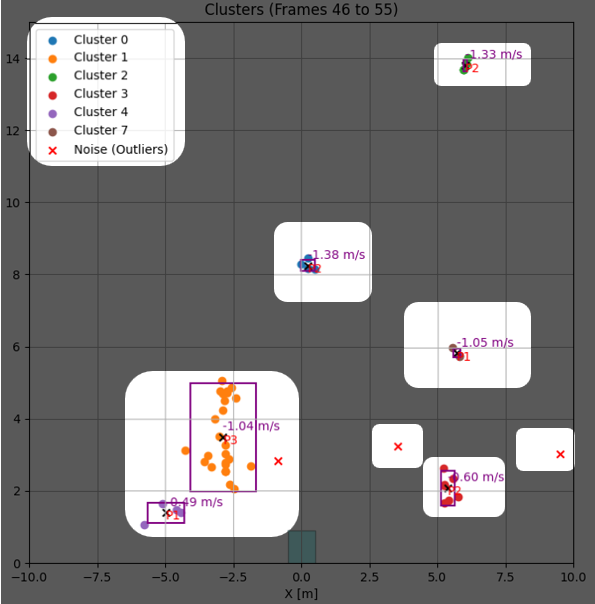
\includegraphics[width=1.0\linewidth]{images/clustering.png}
    \caption{Illustration of the first clustering stage: isolated outliers are discarded, and only candidate clusters remain.}
    \label{fig:first_clustering_stage}
\end{figure}

The resulting process can be expressed as a composition of the two operators:
\begin{equation}
    \mathcal{C}_{\text{final}} = \text{DBSCAN}(\varepsilon_2, \text{MinPts}_2, \; \text{DBSCAN}(\varepsilon_1, \text{MinPts}_1, \; P)),
\end{equation}
where $P$ denotes the raw radar point cloud and $\mathcal{C}_{\text{final}}$ the final set of clusters.  

This formulation highlights the dual role of DBSCAN: first as a noise filter, then as a clustering method.  
By structuring the problem in two passes, the algorithm maintains robustness to noise while achieving finer object separation in dense scenarios.
